\section{Příklad 1}
% Jako parametr zadejte skupinu (A-H)
\prvniZadani{H}

Zřejmě můžeme sečíst napětí zdrojů, protože jsou řazeny sériově a zjistit tak celkové napětí v obvodu.
{\large$$U = U_1 + U_2 = 135\:V + 80\:V = 215\:V$$}
Dále můžeme vypočítat paralelní kombinaci rezistorů $R_7$ a $R_8$: 
{\large$$R_{78} = \frac{R_7*R_8}{R_7 + R_8} = \frac{355*265}{355+265} = 151,7339\:\Omega$$}

Obvod bude nyní vypadat takto: \\

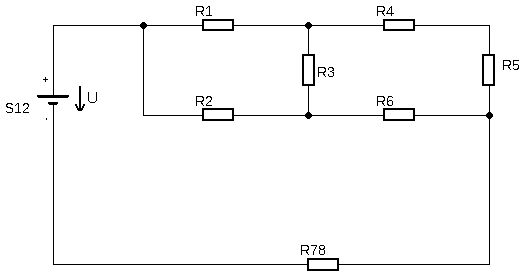
\includegraphics[totalheight=6cm]{fig/1_2.png}

\newpage
Nyní musíme rezistory $R_1$, $R_2$ a $R_3$ převést z trojúhelníkového tvaru na hvězdu. Ekvivalentní rezistory vypočítáme následovně:
{\large$$R_A = \frac{R_1*R_2}{R_1+R_2+R_3} = \frac{680 * 600}{680+600+260} = 264,9351\:\Omega$$}
{\large$$R_B = \frac{R_1*R_3}{R_1+R_2+R_3} = \frac{680*280}{680+600+260} = 114,8052\:\Omega$$}
{\large$$R_C = \frac{R_2*R_3}{R_1+R_2+R_3} = \frac{600*260}{680+600+260} = 101,2987\:\Omega$$}

Tímto nám vznikne tento ekvivalentní obvod: \\

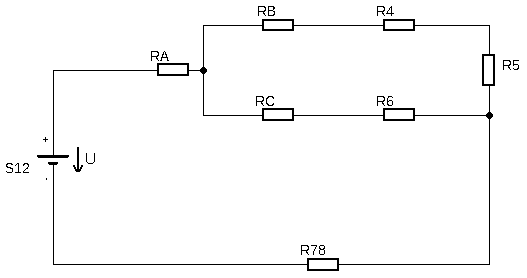
\includegraphics[totalheight=6cm]{fig/1_3.png}

Zjednodušíme si serioparalelní zapojení větví na dva paralelní rezistory:
{\large$$R_{B45} = R_B + R_4 + R_5 = 114,8052 + 310 + 575 = 999,8052\:\Omega$$}
{\large$$R_{C6} = R_C + R_6 = 101,2987 + 870 = 971,2987\:\Omega$$}

Vznikne nám obvod: \\

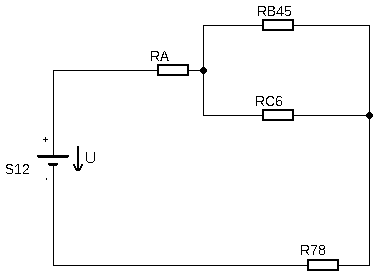
\includegraphics[totalheight=6cm]{fig/1_4.png}

Vypočteme odpor paralelní kombinace nově vzniklých rezistorů:
{\large$$R_{BC456} = \frac{R_{B45} * R_{C6}}{R_{B45} + R_{C6}} = \frac{999,8052 * 971,2987}{999,8052 + 971,2987} = 492,6729\:\Omega$$}
Zůstávají už jen 3 sériové rezistory: \\

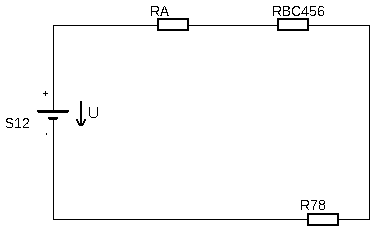
\includegraphics[totalheight=6cm]{fig/1_5.png}

Zjednodušíme obvod pouze na jeden rezistor sečtením těchto rezistorů zapojených do série:
{\large$$R = R_A + R_{BC456} + R_{78} = 264,9351 + 492,6729 + 151,7339 = 909,3419\:\Omega$$}

Finální ekvivalentní obvod: \\

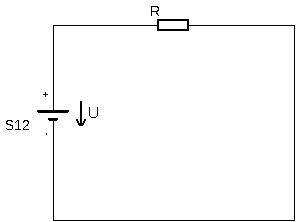
\includegraphics[totalheight=6cm]{fig/1_6.png}

Nyní můžeme vypočítat celkový proud obvodem podle Ohmova zákona:
{\large$$I = \frac{U}{R} = \frac{215}{909,3419} = 236,4347\:mA$$}
\newpage
Nyní, se znalostí celkového proudu U a napětí I, je třeba se postupně dopracovat ke konkrétnímu napětí a proudu na rezistoru $R_5$
Vrátíme se ke 2. kroku zjednodušování a vypočítáme si napětí na serioparalelní kombinaci rezistorů $R_B$, $R_C$, $R_4$, $R_5$ a $R_6$: \\

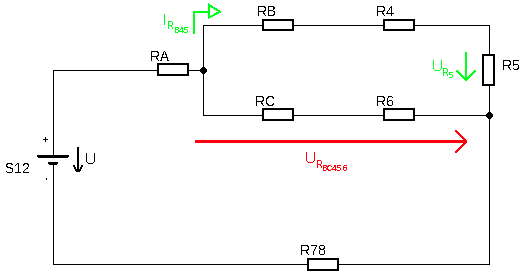
\includegraphics[totalheight=6cm]{fig/1_7.png}

Již víme, že kombinace těchto rezistorů má odpor $R_{BC456} = 492,6729\:\Omega$ 

Napětí tedy vypočítáme podle Ohmova zákona:
{\large$$U_{R_{BC456}} = I * R_{BC456} = 236,4347 * 10^{-3} * 492,6729 = 116,4850\:V$$}

Podle Ohmova zákona nyní můžeme určit proud větví $R_{B45}$:
{\large$$I_{R_{B45}} = \frac{U_{R_{BC456}}}{R_{B45}} = \frac{116,4850 * 10^{-3}}{999,8052} = 116,5077\:mA$$}

A následně napětí přímo na rezistoru $R_5$:
{\large$$U_{R_5} = I_{R_{B45}} * R_5 = 116,5077 * 10^{-3} * 575 = 66,9919\:V$$}

Výsledné napětí a proud na rezistoru $R_5$ tedy je 
{\large$$U_{R_5} = 66,9919\:V$$
$$I_{R_5} = 116,5077\:mA \approx 0,1165\:A$$}